\section{Data Analysis}

\lettrine[nindent=0em,lines=3]{I}n this section, we are going to conduce an analysis on the main characteristics of the features contained in the training dataset. The training set consists of 1126 bad quality samples and 613 good quality samples, then one class is twice as much present as the other. A visualization of how raw features are distributed is shown in Figure \ref{fig:raw}.

\begin{figure}[H]
	\foreach \i in {0,1,...,10}{
		\includegraphics[width=.15\textwidth]{assets/raw_hist\i}
	}
\caption{Raw features distribution of the UCI Wine Quality Dataset}
\label{fig:raw}
\end{figure}

We can observe that features don't have a zero mean, therefore we might consider standardizing them, i.e. centering data and scaling it by the variance, so that the obtained random variable has zero mean and unitary variance. 

In addition, features don't expose a Gaussian trend, with the presence of some outliers.

Therefore, we gaussianize the features, computing the cumulative rank $r(x)$ over the training set 
\begin{align*}
	r(x) = \frac{\sum^N_{i=1} I[x < x_i] + 1}{N + 2}
\end{align*}

being $x_i$ the value of the considered feature for the i-th sample, and transforming the features computing the inverse of the cumulative distribution function $\Phi$ fed with the rank $r(x)$

\begin{align*}
	X_{gauss} = \Phi^{-1} (r(x)) 
\end{align*}

The distribution of the gaussianized features is shown in Figure \ref{fig:gauss}.


Moreover, we provide an analysis of the correlation between the features, exploiting the Pearson product-moment correlation coefficient, defined as

\begin{align*}
	\rho_{X, Y} = \frac{cov(X, Y)} {\sigma_X \sigma_Y}
\end{align*}


\begin{figure}[H]
	\foreach \i in {0,1,...,10}{
		\includegraphics[width=.15\textwidth]{assets/gauss_hist\i}
	}
	\caption{Gaussianized features distribution of the UCI Wine Quality Dataset}
	\label{fig:gauss}
\end{figure}

being $cov(X, Y)$ the covariance matrix of $X$ and $Y$, expressible as the expectation of the product of $X$ and $Y$ centered using their respective mean.

\begin{align*}
	cov(X, Y) = \mathbb{E}[(X - \mu_X)(Y - \mu_Y)]
\end{align*}

The obtained heatmaps among the gaussianized features are shown in Figure \ref{fig:heat}.

\begin{figure}[H]
	\begin{minipage}{\textwidth}
	\hspace{-.2cm}
	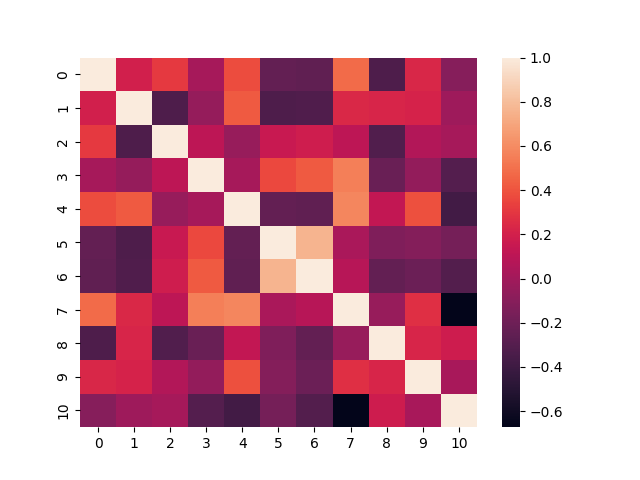
\includegraphics[width=.17\textwidth]{assets/gauss_feat_heat}
	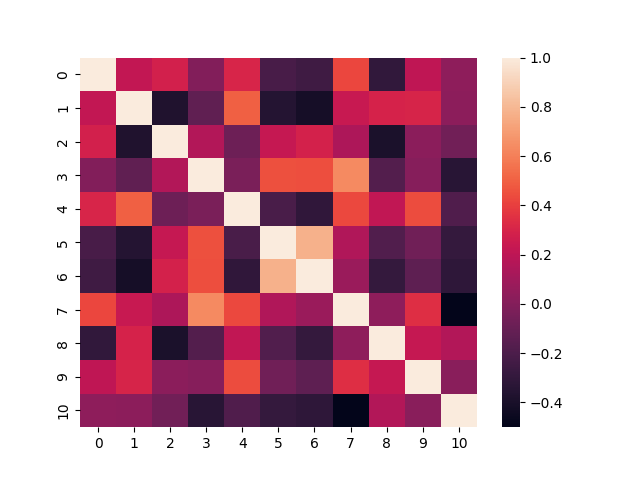
\includegraphics[width=.17\textwidth]{assets/gauss_feat_heat0}
	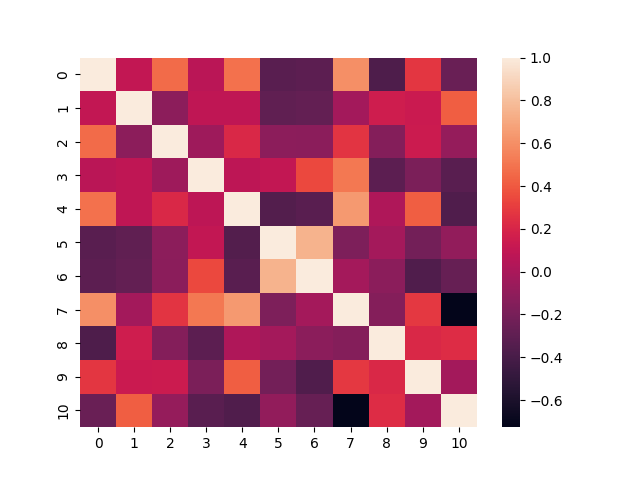
\includegraphics[width=.17\textwidth]{assets/gauss_feat_heat1}
	\end{minipage}

	\caption{Heatmaps among Gaussianized features}
	\label{fig:heat}	
\end{figure}

where we can observe some features are correlated (darker colors in the heatmap), thus exploring dimensionality reduction techniques such as the PCA, could prove beneficial.